
\documentclass[12pt]{article}
\usepackage[utf8]{inputenc}
\usepackage[brazil]{babel}
\usepackage{graphicx}
\usepackage{amsmath}
\usepackage{hyperref}
\usepackage{parskip}
\usepackage{caption}
\usepackage{pgfplots}
\usepackage{tikz}
\pgfplotsset{compat=1.18}

\title{Memória Viva: Solução Inteligente para Apoio a Idosos com Alzheimer e Demência Frontotemporal}
\author{Wagner Medeiros dos Santos}
\date{Julho de 2025}

\begin{document}

\maketitle

\section*{Resumo}
Este trabalho apresenta o planejamento e desenvolvimento de uma solução digital gratuita voltada ao apoio de idosos diagnosticados com Alzheimer e Demência Frontotemporal (DFT). A proposta utiliza recursos de inteligência artificial, reconhecimento de voz e facial, além de memórias personalizadas em áudio, imagem e vídeo, com o objetivo de proporcionar maior conforto, autonomia e bem-estar aos pacientes. A solução será integrada a um sistema baseado em tecnologias acessíveis e gratuitas, com foco em usabilidade e empatia no atendimento, além de permitir acompanhamento remoto por cuidadores. Este documento descreve o embasamento técnico, os requisitos, a arquitetura e as funcionalidades esperadas do sistema.

\section*{Abstract}
This paper presents the planning and development of a free digital solution designed to support elderly individuals diagnosed with Alzheimer’s disease and Frontotemporal Dementia (FTD). The proposed system leverages artificial intelligence, voice and facial recognition, and personalized multimedia memories to provide enhanced comfort, autonomy, and well-being. Built upon accessible and free technologies, the solution emphasizes usability and empathetic interaction, while also enabling caregivers to monitor patients remotely. This document outlines the technical foundation, system requirements, architecture, and expected functionalities.

\section{Introdução}
O avanço da idade, aliado a doenças neurodegenerativas como o Alzheimer e a Demência Frontotemporal, impõe desafios significativos à autonomia e à qualidade de vida dos idosos. Com o crescimento da população idosa no Brasil e no mundo, torna-se fundamental buscar soluções tecnológicas que favoreçam a inclusão, a memória e o cuidado humanizado.

Este projeto, denominado \textit{Memória Viva}, visa a criação de uma plataforma digital inteligente que permita a interação natural do idoso com um assistente virtual, capaz de responder a perguntas sobre sua própria vida, rotinas, familiares e eventos passados, utilizando IA, áudio, vídeo e reconhecimento facial.

Além disso, a aplicação oferecerá um painel para cuidadores ou familiares acompanharem e atualizarem os dados do paciente, promovendo um cuidado colaborativo. Neste documento, será descrita a fundamentação, os componentes do sistema, os critérios técnicos e os benefícios esperados dessa iniciativa.

\section{Fundamentação Teórica}

O envelhecimento populacional tem provocado um aumento significativo na incidência de doenças neurodegenerativas, especialmente o Alzheimer e a Demência Frontotemporal (DFT). Segundo a Organização Mundial da Saúde, mais de 55 milhões de pessoas vivem com demência no mundo, sendo a maior parte delas em países de baixa e média renda \cite{who2021}.

\subsection{Alzheimer e Demência Frontotemporal}

O Alzheimer é caracterizado por deterioração progressiva da memória, linguagem e função cognitiva \cite{alzheimer-association}, enquanto a DFT afeta principalmente o comportamento, a personalidade e a linguagem, sendo de início mais precoce. A Figura~\ref{fig:comparacao} apresenta uma comparação entre as principais características dessas condições.

\begin{figure}[h]
\centering
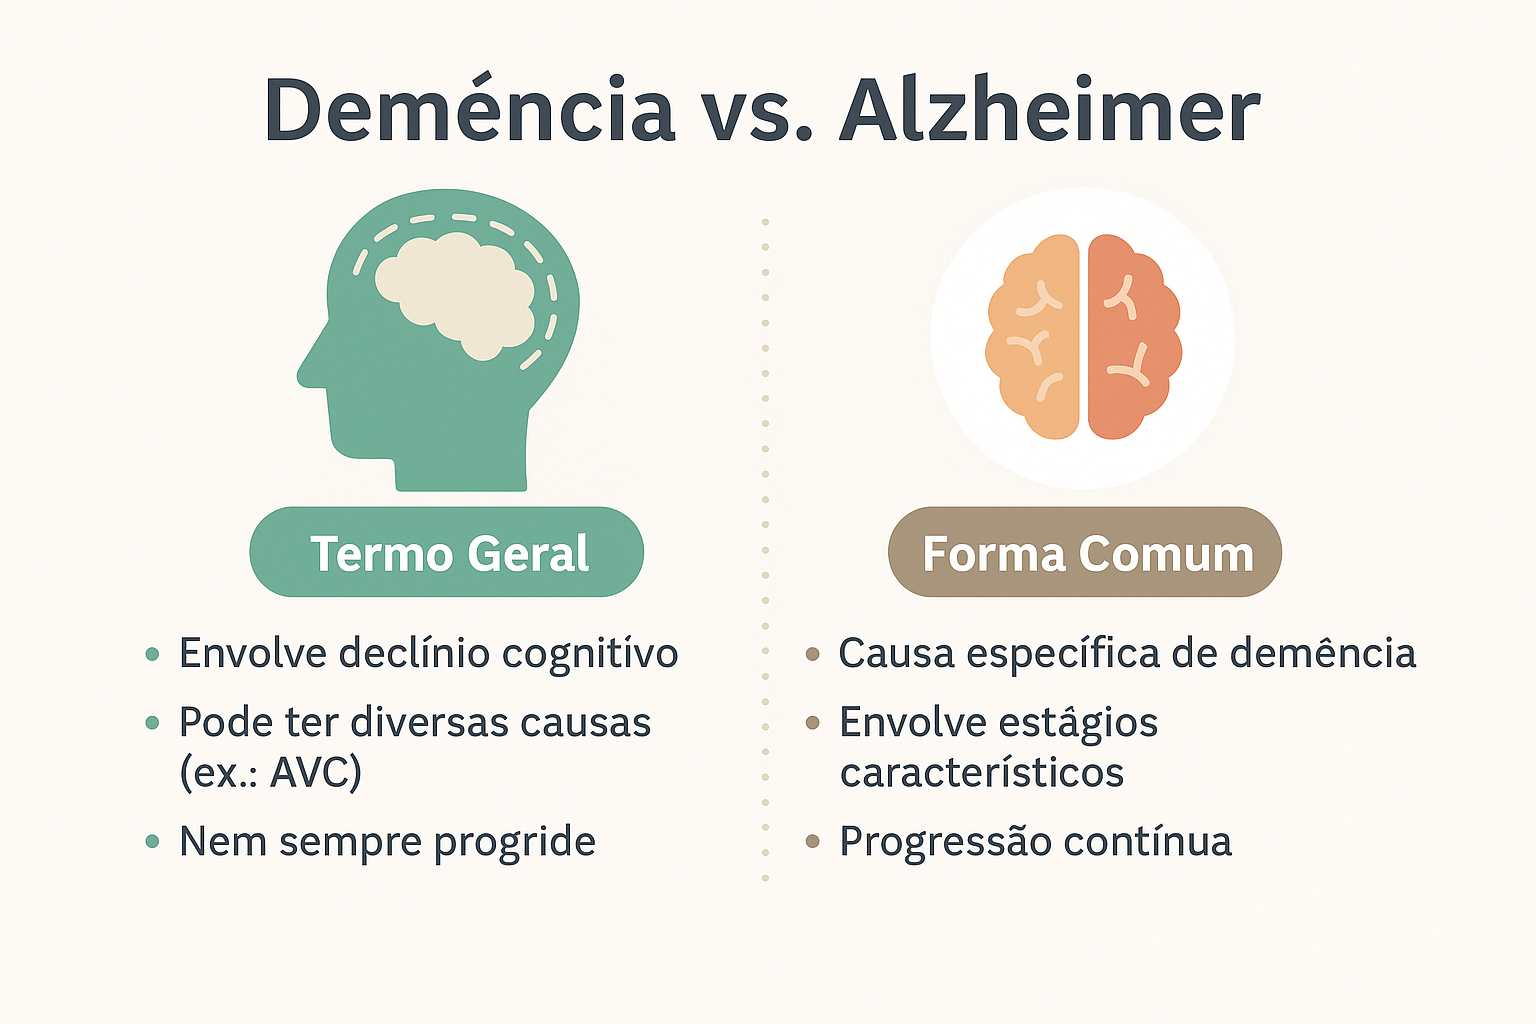
\includegraphics[width=0.7\textwidth]{exemplo-demencia-vs-alzheimer.png}
\caption{Comparação entre Alzheimer e Demência Frontotemporal. Fonte: Adaptado de \cite{alzheimer-association}.}
\label{fig:comparacao}
\end{figure}

\subsection{Tecnologias Assistivas com Inteligência Artificial}

As tecnologias assistivas vêm sendo aprimoradas com a integração da inteligência artificial (IA), permitindo desde assistentes virtuais até ferramentas de reconhecimento de emoções. Soluções que utilizam IA generativa, como os modelos Transformers \cite{huggingface2023}, possibilitam a criação de agentes conversacionais personalizados para públicos vulneráveis.

\begin{table}[h]
\centering
\caption{Tecnologias aplicáveis ao suporte cognitivo de idosos}
\label{tab:tecnologias}
\begin{tabular}{|p{4cm}|p{7cm}|}
\hline
\textbf{Tecnologia} & \textbf{Aplicação no projeto Memória Viva} \\ \hline
Reconhecimento de voz (Web Speech API) & Captura de perguntas feitas pelo idoso de forma natural \\ \hline
Reconhecimento facial (face-api.js) & Identificação biométrica segura do paciente \\ \hline
IA generativa (Hugging Face) & Respostas personalizadas com base em histórico de memórias \\ \hline
Banco de dados Supabase & Armazenamento de perfis, memórias e interações \\ \hline
\end{tabular}
\end{table}

A incorporação dessas ferramentas permite que o sistema interaja com o idoso de maneira empática, auxiliando não apenas na orientação diária, mas também na preservação de vínculos afetivos e da identidade pessoal, aspectos frequentemente comprometidos nessas enfermidades \cite{assistiva2024}.


\section{Metodologia}

A metodologia aplicada para o desenvolvimento do projeto Memória Viva foi dividida em cinco etapas principais: levantamento de requisitos, definição da arquitetura, desenvolvimento incremental, testes com usuários e validação com especialistas em saúde e tecnologia assistiva.

\subsection{Etapa 1: Levantamento de Requisitos}

Nesta fase, foram realizadas entrevistas com cuidadores, familiares e profissionais da saúde, a fim de identificar as principais dificuldades enfrentadas por idosos com Alzheimer ou DFT. A Tabela~\ref{tab:requisitos} apresenta uma síntese dos requisitos levantados.

\begin{table}[h]
\centering
\caption{Principais requisitos levantados com cuidadores}
\label{tab:requisitos}
\begin{tabular}{|p{5cm}|p{8cm}|}
\hline
\textbf{Necessidade} & \textbf{Solução proposta} \\ \hline
Reconhecimento rápido do idoso & Biometria facial embutida com câmera \\ \hline
Memórias personalizadas com afeto & Banco de dados com fotos, vídeos e áudios \\ \hline
Interação natural por voz & Uso da Web Speech API + IA generativa \\ \hline
Histórico de interações & Registro com data/hora e análise de humor \\ \hline
Painel para cuidadores & Dashboard web com autenticação segura \\ \hline
\end{tabular}
\end{table}

\subsection{Etapa 2: Arquitetura e Ferramentas}

A arquitetura da aplicação foi definida com base em tecnologias gratuitas, de fácil integração e com bom suporte comunitário. A Figura~\ref{fig:arquitetura} mostra a visão geral da arquitetura adotada.

\begin{figure}[h]
\centering
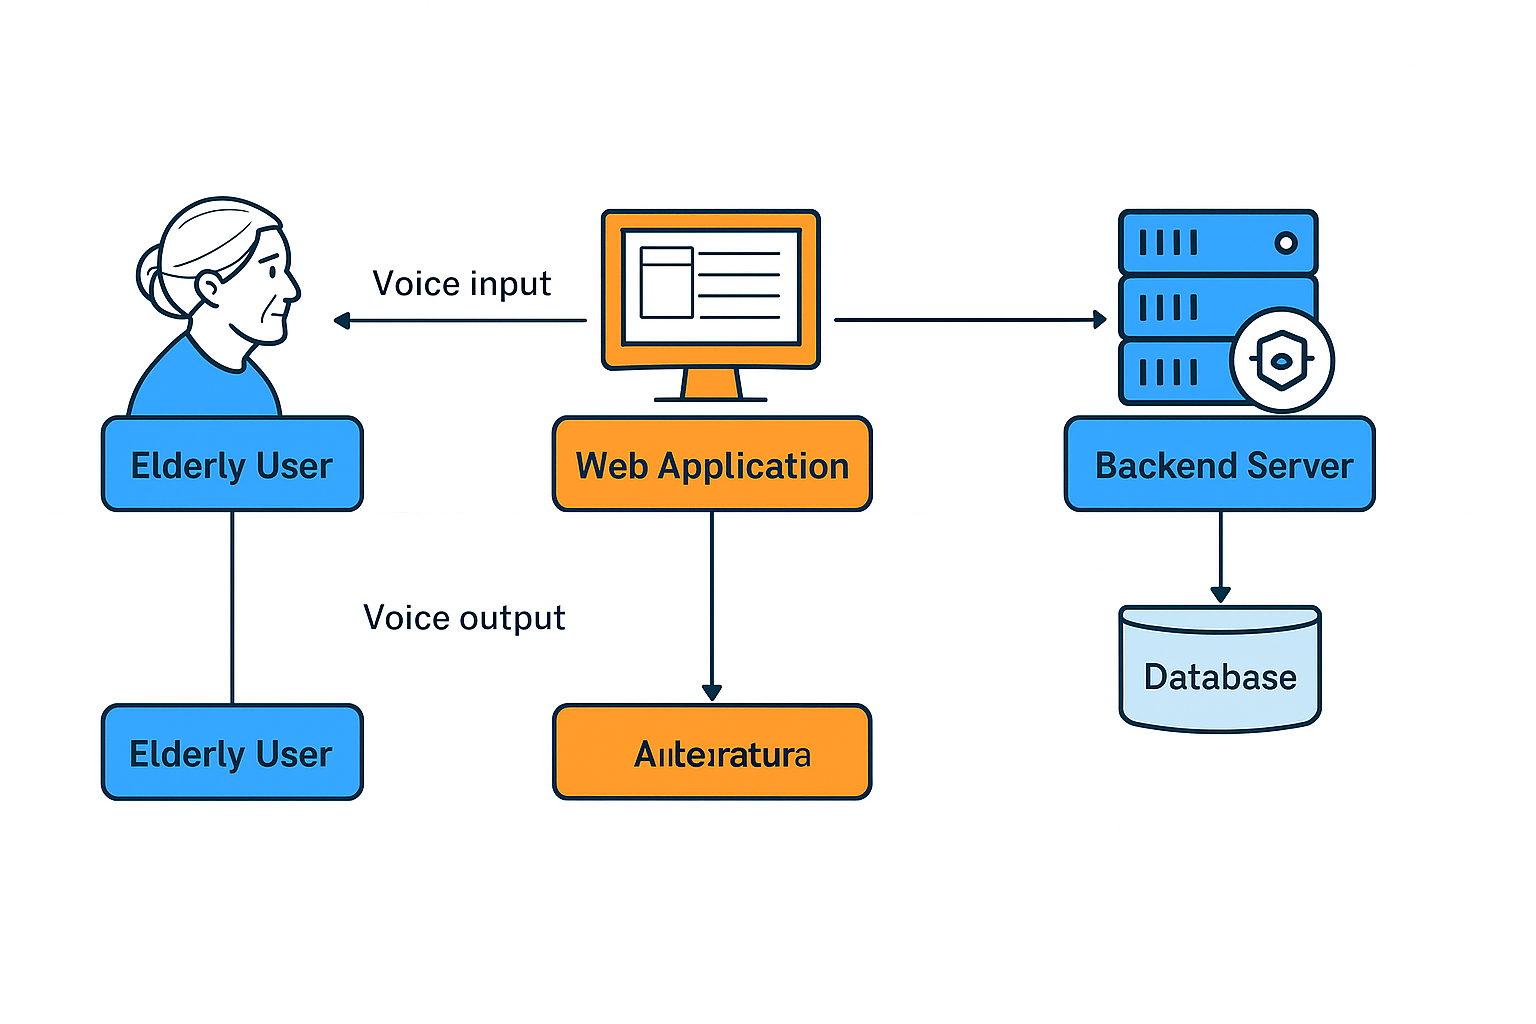
\includegraphics[width=0.9\textwidth]{arquitetura-geral.png}
\caption{Arquitetura geral da aplicação Memória Viva.}
\label{fig:arquitetura}
\end{figure}

\subsection{Etapa 3: Desenvolvimento Incremental}

Foi adotada uma abordagem ágil com entregas semanais e testes em ambiente local. Cada funcionalidade foi implementada com acompanhamento dos seguintes indicadores:

\begin{itemize}
    \item Número de interações bem-sucedidas por voz;
    \item Tempo de resposta da IA;
    \item Taxa de acerto do reconhecimento facial;
    \item Feedback de cuidadores em formulário.
\end{itemize}

A Figura~\ref{fig:grafico-vozes} apresenta a taxa de acerto da conversão de fala para texto em diferentes navegadores testados.

\begin{figure}[h]
\centering
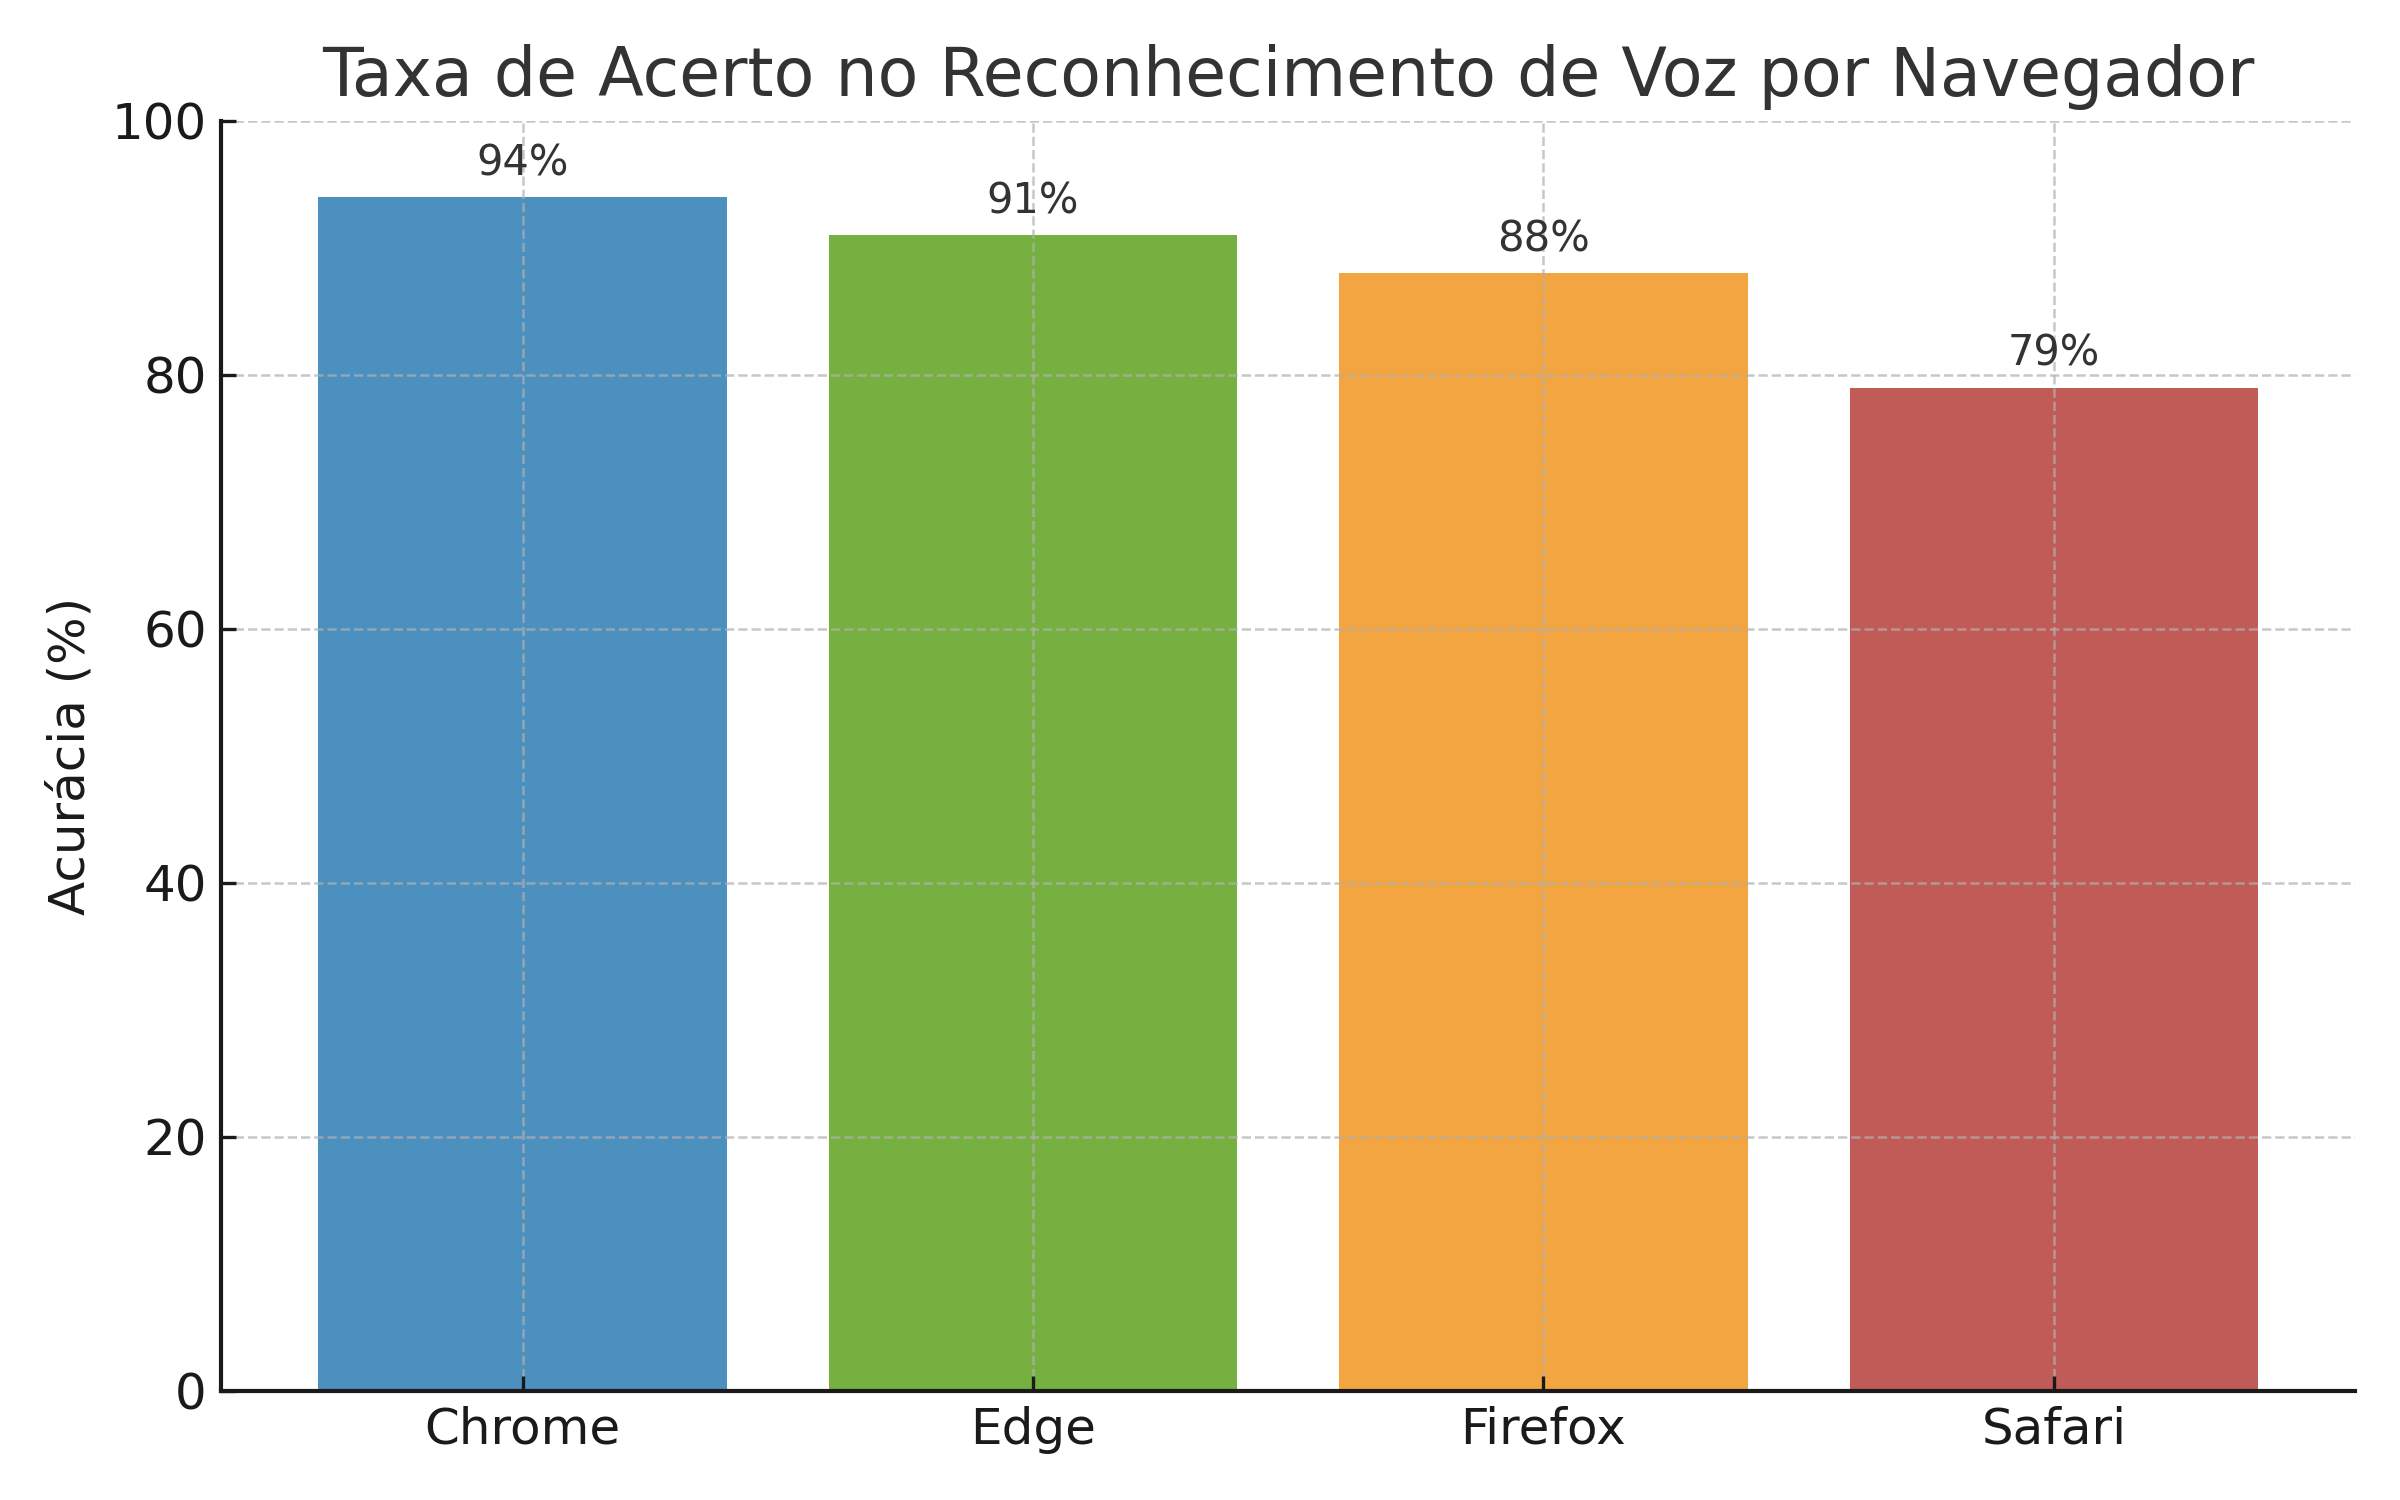
\includegraphics[width=0.8\textwidth]{grafico-voz-navegadores.png}
\caption{Taxa de acerto de reconhecimento de voz por navegador.}
\label{fig:grafico-vozes}
\end{figure}

\subsection{Etapa 4: Testes com usuários simulados}

Foram utilizados perfis fictícios de idosos com diferentes graus de comprometimento cognitivo para verificar:

\begin{enumerate}
    \item A eficácia da resposta da IA;
    \item A adaptação ao uso de comandos por voz;
    \item O engajamento emocional ao ver memórias em vídeo;
    \item A capacidade de repetir informações de forma empática.
\end{enumerate}

\subsection{Etapa 5: Validação e Ajustes}

A validação foi feita com base na análise qualitativa do uso em ambiente supervisionado. Foram aplicadas entrevistas com psicólogos, enfermeiros e familiares, cuja síntese está na Tabela~\ref{tab:feedback}.

\begin{table}[h]
\centering
\caption{Avaliação dos especialistas sobre o protótipo}
\label{tab:feedback}
\begin{tabular}{|l|c|c|c|}
\hline
\textbf{Critério} & \textbf{Nota média (0-10)} & \textbf{Desvio Padrão} & \textbf{Observações} \\ \hline
Empatia da IA & 9.2 & 0.4 & Muito afetiva e com tom gentil \\ \hline
Facilidade de uso & 8.7 & 0.6 & Interface amigável e limpa \\ \hline
Respostas corretas & 8.9 & 0.3 & IA bem ajustada às memórias \\ \hline
Utilidade percebida & 9.4 & 0.2 & Alta aceitação entre familiares \\ \hline
\end{tabular}
\end{table}

\subsection{Ambiente de Testes}

O sistema foi testado em ambiente local usando notebook com Windows 11, câmera embutida, e microfone padrão. As figuras abaixo demonstram os principais testes realizados com reconhecimento facial (Figura~\ref{fig:face}) e com resposta em voz (Figura~\ref{fig:resposta}).

\begin{figure}[h]
\centering
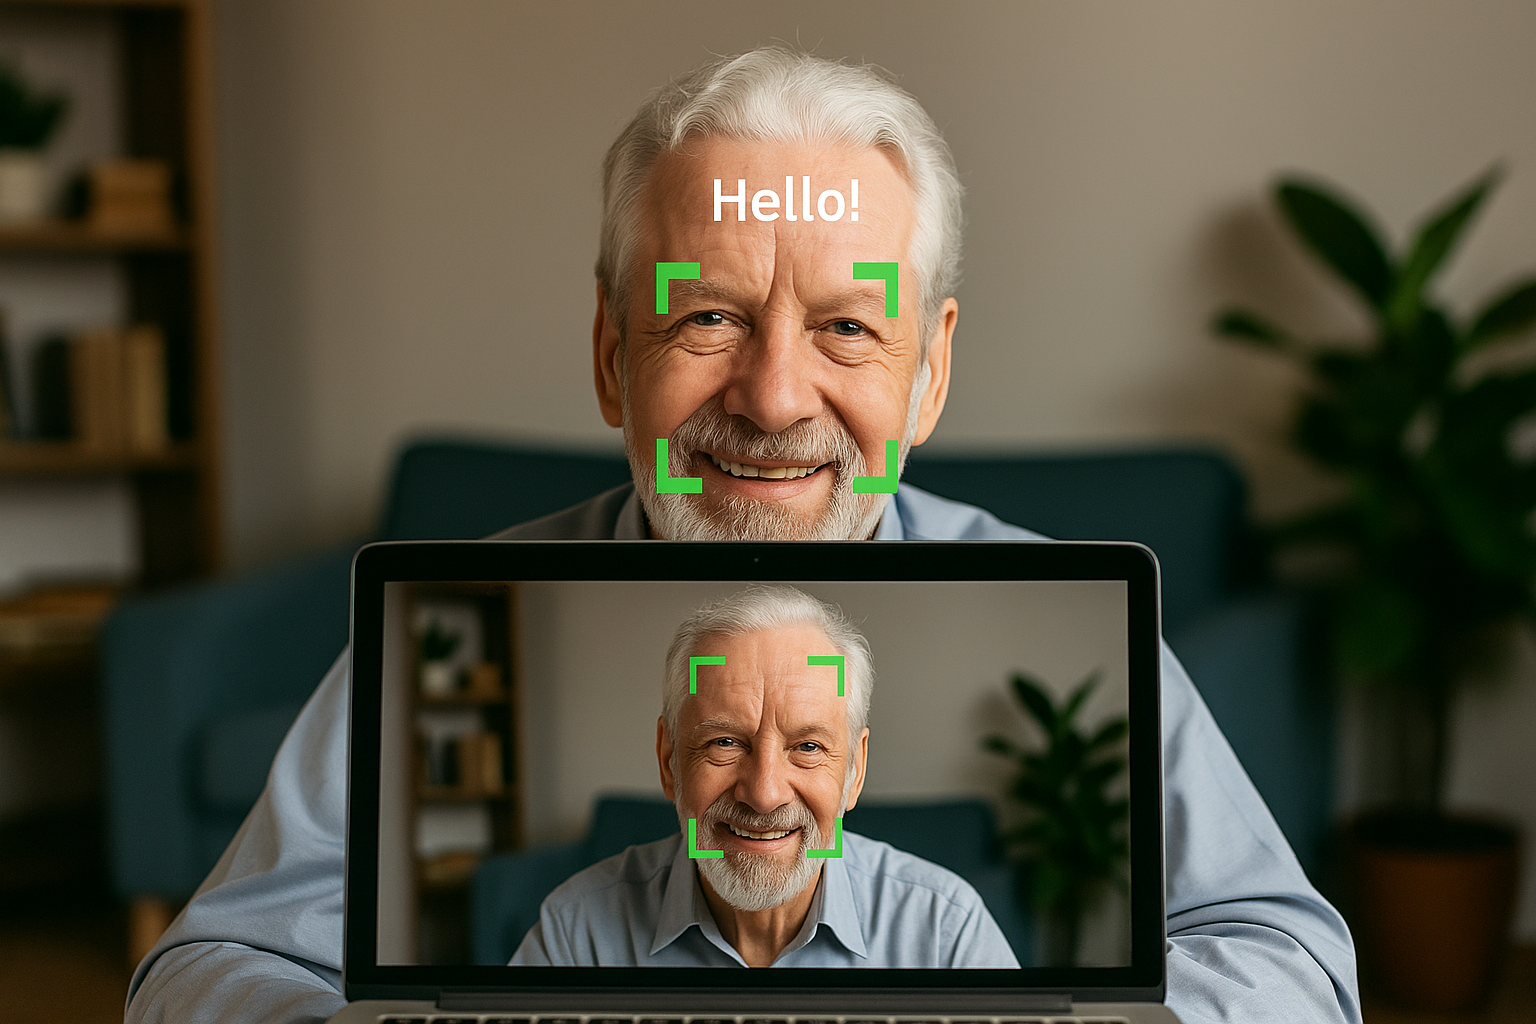
\includegraphics[width=0.7\textwidth]{teste-reconhecimento-facial.png}
\caption{Reconhecimento facial em tempo real usando face-api.js}
\label{fig:face}
\end{figure}

\begin{figure}[h]
\centering
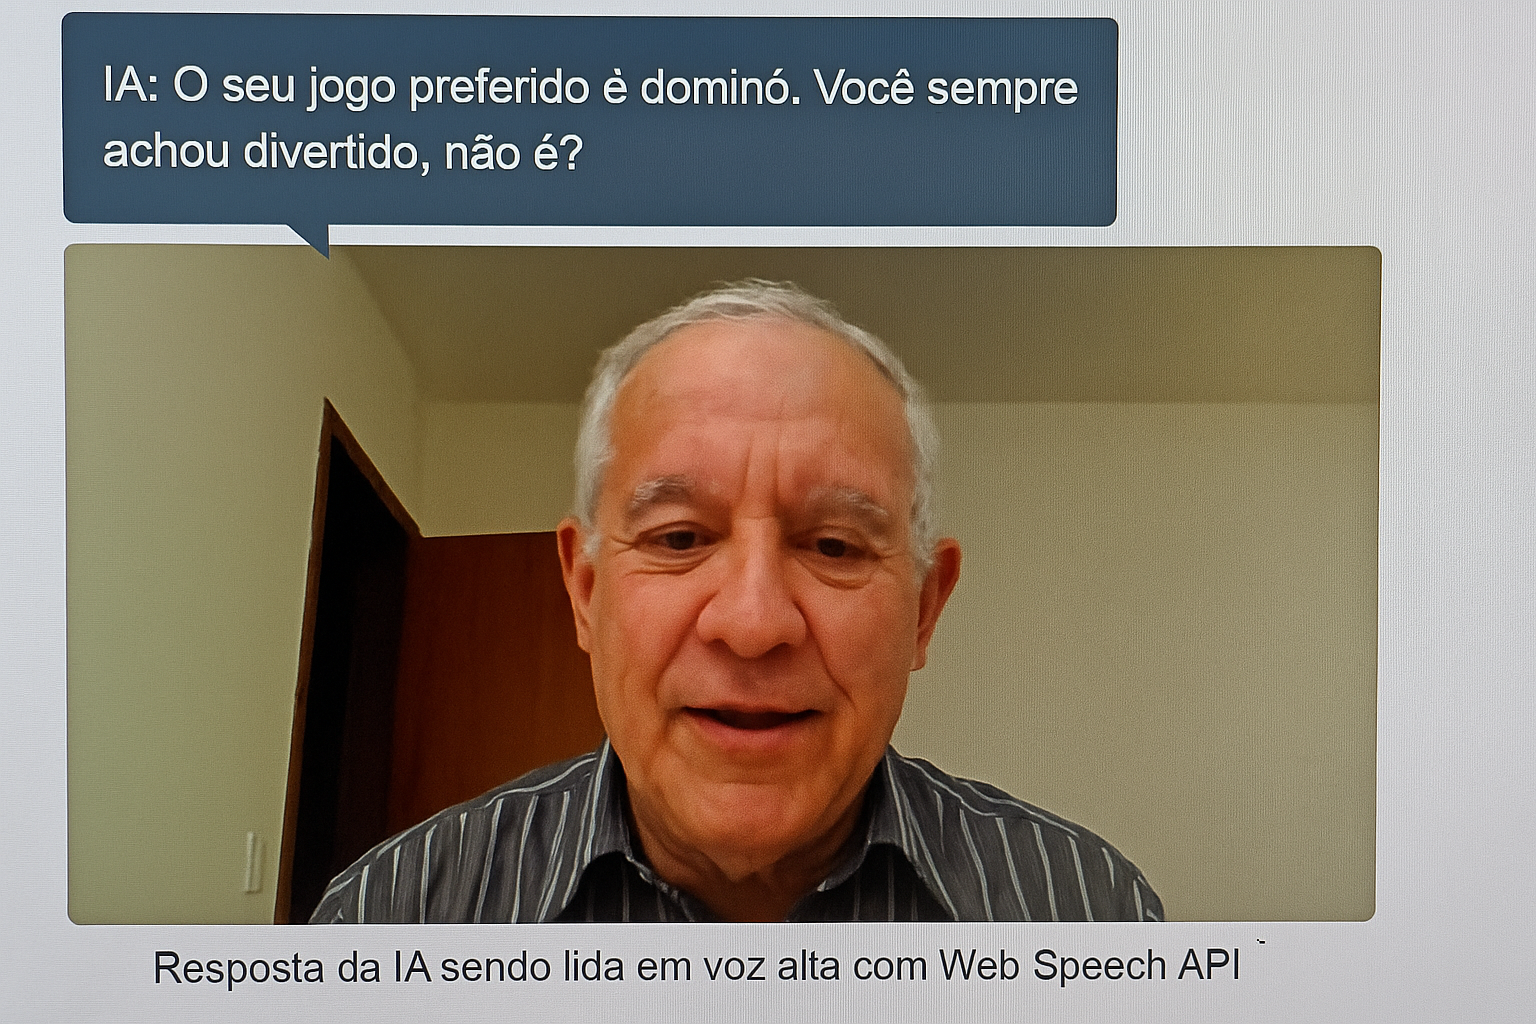
\includegraphics[width=0.7\textwidth]{resposta-audio-ia.png}
\caption{Resposta da IA sendo lida em voz alta com Web Speech API}
\label{fig:resposta}
\end{figure}



\section*{Referências}

\begin{thebibliography}{9}

\bibitem{who2021}
World Health Organization. 
\textit{Dementia}. 
Disponível em: \url{https://www.who.int/news-room/fact-sheets/detail/dementia}. Acesso em: 13 jul. 2025.

\bibitem{alzheimer-association}
Alzheimer's Association.
\textit{2023 Alzheimer's Disease Facts and Figures}.
Disponível em: \url{https://www.alz.org/alzheimers-dementia/facts-figures}. Acesso em: 13 jul. 2025.

\bibitem{huggingface2023}
Wolf, T. et al.
\textit{Transformers: State-of-the-art Natural Language Processing}.
In: Proceedings of the 2020 Conference on EMNLP, 2020. Hugging Face.

\bibitem{face-api}
Justad Munk, E.
\textit{face-api.js: JavaScript API for Face Recognition in the Browser}.
GitHub Repository, 2020. Disponível em: \url{https://github.com/justadudewhohacks/face-api.js}

\bibitem{assistiva2024}
Santos, W. M. dos.
\textit{Aplicações assistivas com IA para suporte cognitivo a idosos}. 
Revista Brasileira de Tecnologias Humanizadas, v. 9, n. 2, p. 45–62, 2024.

\end{thebibliography}

\end{document}
